 \chapter{Antecedentes}

Este capítulo describe el proceso de adquisición de conocimientos necesarios para poder llevar a cabo el proceso de diseño arquitectónico y de construcción o implementacíon de la aplicación. De esta fomra se puede realizar una planificación mas cercana a la realidad y partir de unos conocimientos mínimos para empezar a elaborar el proyecto.
	
\minitoc
	
\section{Go.JS}

Go.JS~\cite{gojs} es una biblioteca de JavaScript para implementar editores gráficos dentro de interfaces web. GoJS facilita la implementación de tareas tales como definición de símbolos gráficos, gestión de paletas de símbolos, arrastrar y soltar (\emph{drag and drop}), copiar y pegar, edición de etiquetas de texto asociadas a símbolos gráficos, menús contextuales, función de deshacer o la gestión de eventos de ratón, entre muchos otros elementos.

Para ilustrar el funcionamiento de GoJS, a continuación se mostrará a modeo de ejemplo cómo crear un editor gráfico para diseñar unos pseudo diagramas de flujo compuestos por círculos y rectángulos interconectados por flechas. Dicho editor se muestra en la Figura~\ref{fig:gojssample}.

\begin{figure}[!tb]
	\centering
	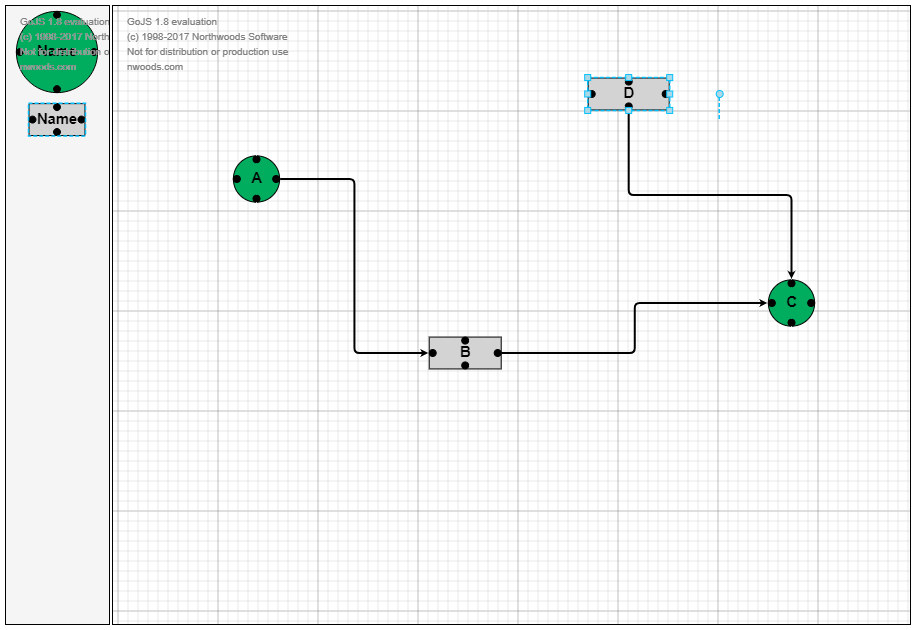
\includegraphics[width=\linewidth]{gojssample.png}
	\caption{Editor gráfico creado en GoJS}
    \label{fig:gojssample}
\end{figure}

Para comenzar, cabe destacar que, es necesario reservar dos secciones de la página HTML que lo contiene. Una sección albergará la paleta con los elementos gráficos del editor, que en este caso serán sólo el círculo y el rectángulo, y otra sección para el diagrama o lienzo sobre el que se depositarán los elementos gráficos.

A continuación, se debe realizar una serie de acciones a nivel de Javascript para proporcionar tanto a la paleta de dibujo como al área de dibujo del comportamiento deseado. En primer lugar, crearemos una variable \texttt{\$} que dé acceso al entorno GoJS. Esto se realiza mediante la llamada a la sentencia \texttt{make} de librería \emph{GraphObject} de GoJS (Figura~\ref{fig:asignacionDollar}, Línea~1).

\begin{figure}[!tb]
	\centering
	\begin{lstlisting}[language=JavaScript]
	var $ = go.GraphObject.make;\end{lstlisting}
	\caption{Asignación de la variable \texttt{\$}}
	\label{fig:asignacionDollar}
\end{figure}

Seguidamente, se personaliza la sección HTML reservada al diagrama, denominada \texttt{myDiagramDiv} (Figura~\ref{fig:creacionDiagrama}, Líneas~01-13), asignándole un \emph{grid} o cuadrícula de fondo (Figura~\ref{fig:creacionDiagrama}, Líneas~04-09), especificando los colores de las líneas de la cuadrícula (mediante la propiedad \emph{stroke}) y dándole la capacidad de poder arrastrar elementos sobre él (Figura~\ref{fig:creacionDiagrama}, Línea~10).

\begin{figure}[!tb]
	\centering
	\begin{lstlisting}[language=JavaScript]
	myDiagram =
		$(go.Diagram, "myDiagramDiv",
		{
			grid: $(go.Panel, "Grid",
				$(go.Shape, "LineH", { stroke: "lightgray", strokeWidth: 0.5 }),
				$(go.Shape, "LineH", { stroke: "gray", strokeWidth: 0.5, interval: 10 }),
				$(go.Shape, "LineV", { stroke: "lightgray", strokeWidth: 0.5 }),
				$(go.Shape, "LineV", { stroke: "gray", strokeWidth: 0.5, interval: 10 })
			),
			allowDrop: true,
		}
	);\end{lstlisting}
	\caption{Creación de un diagrama en GoJS}
	\label{fig:creacionDiagrama}
\end{figure}

A continuación deberemos definir lo que en GoJS se conoce como la \emph{plantilla de nodos} o \emph{node template}. Esta plantilla define el comportamiento genérico de todos los nodos que compondrán nuestro diagrama. Estos nodos, en nuestro caso, serán rectángulos y círculos. La Figura~\ref{fig:patronNodo} muestra cómo se crea el patrón que servirán de esqueleto para todos los nodos de nuestro diagrama. 

\begin{figure}[!tb]
	\centering
	\begin{lstlisting}[language=JavaScript]
	myDiagram.nodeTemplate =
		$(go.Node, "Spot",
		{ 
			locationSpot: go.Spot.Center 
		},
		new go.Binding("location").makeTwoWay(go.Point.stringify),
		{ 
			selectable: true, 
			selectionAdornmentTemplate: nodeSelectionAdornment 
		},
		{ 
			resizable: true, 
			resizeObjectName: "PANEL", 
			resizeAdornmentTemplate: nodeResizeAdornment 
		},
		{ 
			rotatable: true, 
			rotateAdornmentTemplate: nodeRotateAdornment 
		},
	
		$(go.Panel, "Auto",
		{ 
			name: "PANEL" 
		},
		$(go.Shape,
		{
			portId: "",
			fromLinkable: true, toLinkable: true, cursor: "pointer",
		},
		new go.Binding("figure"),
		new go.Binding("fill")),
		$(go.TextBlock,
		{
			maxSize: new go.Size(50, 50),
			editable: true
		},
		new go.Binding("text").makeTwoWay())
		)
	);\end{lstlisting}
\caption{Declaración del patrón del Nodo}
\label{fig:patronNodo}
\end{figure}

Para crear la definición un nodo lo primero es declarar el nodo con \texttt{\$(go.Node} (Figura~\ref{fig:patronNodo},~Línea~2).
A continuación, especificamos, mediante la definición de ciertas propiedades, cómo se comportará el nodo (Figura~\ref{fig:patronNodo}, Líneas~5-24). En nuestro caso, se indica que los nodo, con carácter general, podrán ser seleccionados, redimensionados y rotados (Figura~\ref{fig:patronNodo}, Líneas~7-19, respectivamente). Se establece que los nodos aparecerán localizados por defecto en el centro del diagrama en el momento de su creación (Figura~\ref{fig:patronNodo}, Línea~4).
Además, se indica que la propiedad \texttt{location}, que establece la posición del nodo, queda expuesta para su modificación desde el exterior (Figura~\ref{fig:patronNodo}, Línea~04).

Siempre que se crea un nodo, se reserva un espacio sobre el que se van a situar los diferentes elementos del nodo. En nuestro ejemplo, este espacio recibe el nombre de \emph{panel}(Figura~\ref{fig:patronNodo}, Línea~21). El panel actúa como contenedor de la figura (\emph{shape}) (Figura~\ref{fig:patronNodo}, Línea~25), que es la encargada de definir la forma del nodo. En nuestro caso, dicho panel podrá poseer diferentes formas (como serán el circulo y el rectángulo) y colores gracias a los \emph{bindings}, que son los que hacen que estas propiedades sean modificables programáticamente (Figura~\ref{fig:patronNodo}, Líneas~30-31). Además, cada nodo poseerá un identificador propio, denominado \emph{portId} (Figura~\ref{fig:patronNodo}, Línea~27) y todos los nodos pueden recibir conexiones tanto de entrado como de salida (\emph{toLinkable} y \texttt{fromLinkable}) (Figura~\ref{fig:patronNodo}, Línea~28). Por último, cada nodo poseerá una etiqueta de texto que permitirá especificar su nombre, el cual también puede ser modificado externamente (Figura~\ref{fig:patronNodo}, Líneas~32-38).

Una vez definidas las propiedades básicas de un nodo, el siguiente paso es definir cómo enlazar dichos nodos. Para ello debemos definir dos elementos: \emph{puertos} y \emph{enlaces}. Los enlaces son los elementos que permiten conectar nodos, y los puertos de un nodo son los puntos de dicho nodo desde donde puede partir un enlace o a dónde puede llegar un enlace.  En la Figura~\ref{fig:gojssample}, estos puertos aparecen aparecen como unos círculos negros en los extremos de las figuras.

\begin{figure}[!tb]
	\centering
	\begin{lstlisting}[language=JavaScript]
	function makePort(name, spot) {
		return $(go.Shape, "Circle",
		{
			desiredSize: new go.Size(7, 7),
			alignment: spot,
			alignmentFocus: spot,
			portId: name,
			fromLinkable: true, toLinkable: true,
			cursor: "pointer"
		});
	}\end{lstlisting}
	\caption{Función MakePort}
	\label{fig:funcionMakeport}
\end{figure}
	
Para añadir puertos a los nodos se ha creado una función una función llamada \emph{makePort}, la cual se muestra en la Figura~\ref{fig:funcionMakeport}. Este fragmento de código define un puerto como una forma circular con un identificador (Figura~\ref{fig:funcionMakeport}, Línea~07), una posición (Figura~\ref{fig:funcionMakeport}, Líneas~05-06) y un tamaño (Figura~\ref{fig:funcionMakeport}, Línea~04). Finalmente, usando esta función, añadimos cuatro llamadas a a misma al final de la plantilla de nodos, con el objeto de crear un puerto a cada lado del eje de cada nodo (Figura~\ref{fig:patronNodoFinal}, Línea~04).

\begin{figure}[!tb]
	\centering
	\begin{lstlisting}[language=JavaScript]
	myDiagram.nodeTemplate =
		$(go.Node, "Spot",
		{ locationSpot: go.Spot.Center },
        ...
		makePort("T", go.Spot.Top),
		makePort("L", go.Spot.Left),
		makePort("R", go.Spot.Right),
		makePort("B", go.Spot.Bottom)
	);\end{lstlisting}
	\caption{Patrón Nodo con Puertos}
	\label{fig:patronNodoFinal}
\end{figure}

Una vez definidos los puertos, especificamos cómo se comportarán los enlaces entre nodos (Figura~\ref{fig:patronlink}). En nuestro caso, se declara que los enlaces irán de un nodo principal \texttt{isPanelMain} a uno secundario,  se efine el grosor del enlace y se establece que el enlace poseerá una flecha al final del mismo (\emph{toArrow: "Standard"}).

\begin{figure}[!tb]
	\centering
	\begin{lstlisting}[language=JavaScript]
	myDiagram.linkTemplate =
		$(go.Link,
			$(go.Shape,
			{ isPanelMain: true, strokeWidth: 2 }),
			$(go.Shape,
			{ toArrow: "Standard", stroke: null }
		)
	)\end{lstlisting}
\caption{Declaración del patrón del Link}
\label{fig:patronlink}
\end{figure}


\begin{figure}[!tb]
	\centering
\begin{lstlisting}[language=JavaScript]
myPalette =
	$(go.Palette, "myPaletteDiv",
	{
		nodeTemplateMap: myDiagram.nodeTemplateMap,
		model: new go.GraphLinksModel([
			{ 
				text: "Name", 
				figure: "Circle", 
				fill: "#00AD5F" 
			},
			{ 
				text: "Name", 
				figure: "Rectangle", 
				fill: "lightgray" 
			}
			])
		}
);\end{lstlisting}
\caption{Creación de la Paleta de Nodos}
\label{fig:paletaNodos}
\end{figure}

Por último, se procede a crear la paleta que contendrá los círculos y los rectángulos, tal como se muestra en la Figura~\ref{fig:paletaNodos}. Como se puede observar, la paleta se sitúa sobre una sección HTML denominada \emph{myPalleteDiv} (Figura~\ref{fig:paletaNodos}, Línea~XX), la cual fue reservada con anterioridad. Para la definición de los nodos que estarán dentro de la paleta se utiliza el mismo patrón e nodos creado con anterioridad (Figura~\ref{fig:paletaNodos}). Finalmente, por último, se declara el \emph{modelo}, que es el conjunto de figuras concretas que poseerá dicha paleta. Para crear los elementos del modelo, se instancia la plantilla de nodos y se cambian sus propiedades con objeto de crear objetos diferentes. En nuestro caso, creamos círculo de color verde (Figura~\ref{fig:paletaNodos}, Línea~06) y rectángulos de color gris (Figura~\ref{fig:paletaNodos}, Línea~07), ambos con \texttt{Name} como nombre por defecto, el cual podrá ser luego editado.

Una vez definidos estos elementos, nuestro editor gráfico queda implementado, y GoJS se encargará de dibujar la paleta y el diagrama, así como, de pintar los elementos sobre el área de dibujo cuando éstos sean seleccionados en la paleta, permitiendo arrastrarlos, redimensionarlos o renombrarlos, entre otras funciones.

\section{Patrón \emph{Model-View-Presenter (MVP)}}
\label{sec:mvp}

%% Detallar aquí brevemente y con claridad, a ser posible, utilizando una figura
%% para ello, el funcionamiento del patrón MVP.
\begin{figure}[H]
	\centering
	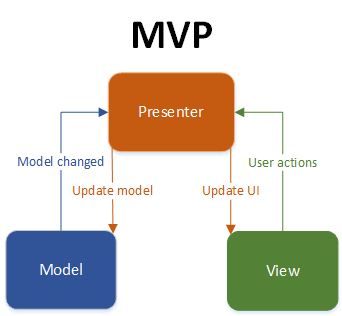
\includegraphics[width=0.6\linewidth]{mvp.png}
	\caption{Patrón Modelo-Vista-Presentador}\label{fig:mvp}
\end{figure}

Este patrón esta orientado a crear interfaces de usuario y su objetivo es separar la lógica de la aplicación de los detalles estéticos de la interfaz. Se compone de tres módulos independientes: \emph{modelo}, \emph{vista} y \emph{presentador} (ver Figura~\ref{fig:mvp}).

%% Poner Figura  


El \emph{modelo} es el encargado de gestionar los datos de la aplicación, y que de alguna forma serán mostrados al usuario. La \emph{vista} es una interfaz de usuario, normalmente gráfica, que se encarga de mostrar datos al usuario de la manera más amigable posible. Por último el presentador se sitúa entre el \emph{Modelo} y la \emph{Vista} y se encarga de conectar ambos elementos. Los eventos realizados sobre la interfaz de usuario se delegan en el presentador, que es el que decide qué cambios se deberán realizar sobre la interfaz gráfica. Para ello puede acceder a datos al modelo, o solicitar la modificación de los mismos. 

De esta forma se separa lo que es la lógica de navegación y procesamiento de eventos de los detalles de cómo se organiza exactamente una interfaz de usuario. De este modo, se aisla dicha lógica de cambios estéticos que pudiesen producrise en dicha interfaz. 

La siguiente sección mostrará como \emph{Vaadin}, un framework para el desarrollo de aplicaciones web, implementa de una manera concreta este patrón.

 




\section{Vaadin}
 		


\emph{Vaadin}~\cite{vaadin} es un \textbf{framework} para el desarrollo de aplicaciones \emph{web} avanzadas, también conocidas como \emph{Rich-Internet Applications (RIA)}~\cite{ria}. El objetivo del paradigma \emph{RIA} es desarrollar aplicaciones \emph{web} con interfaces avanzadas que les haga asemejarse a las aplicaciones de escritorio. La principal ventaja que aporta \emph{Vaadin} es que permite escribir aplicaciones en código Java, como si fuesen de escritorio, y luego este código es transformado para que funcione en tecnologías web como HTML (HyperText Markup Language)~\cite{html}, CSS (Cascading Style Sheets)~\cite{css}, Javascript~\cite{javascript}, HTTP (Hypertext Transfer Protocol)~\cite{http} o AJAX (Asynchronous JavaScript and XML)~\cite{ajax}.

Una de las características diferenciadores de \texttt{Vaadin} es que, al contrario de las librerías de JavaScript tradicionales, \emph{Vaadin} también contempla la parte del servidor, por lo se generan tanto las llamadas al servidor desde la interfaz gráfica (\emph{front-end}) como la recepción y tratamiento de esas llamadas en la parte del servidor (\emph{back-end}).



 	
 \subsection{Ejemplo Vaadin}
 	
\begin{figure}[!tb]
	\centering
	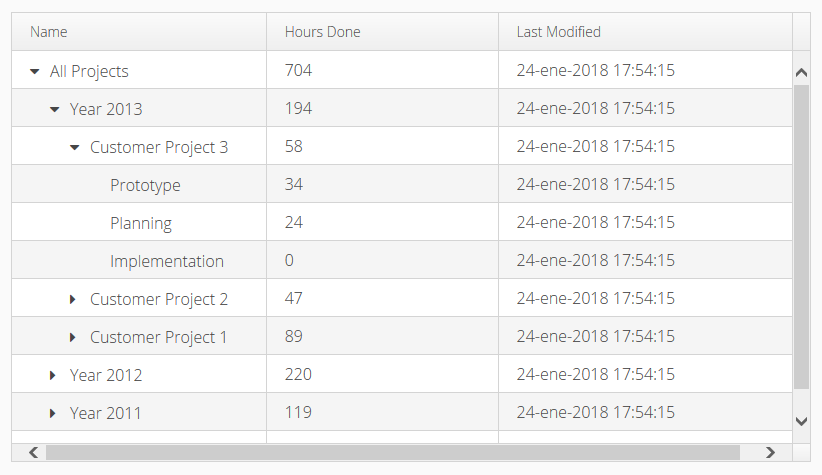
\includegraphics[width=\linewidth]{vaadinExampleImage.png}
	\caption{Árbol de Proyectos}
	\label{fig:vaadinExampleImage}
\end{figure}

A continuación, se explica un ejemplo de contrucción de una jerarquía de tareas propias en la gestión de proyectos por parte de un Jefe de Proyecto (Figura~\ref{fig:vaadinExampleImage}).

El proyecto creado para realizar el ejemplo se compone de una interfaz de usuario (Figura~\ref{fig:uiVaadin}) la cuál utiliza un componente llamado TreeGrid  (será explicado posteriormente,Figura~\ref{fig:treeGrid}) y un contenedor de datos (Figura~\ref{fig:demoContainer}).

Para entrar en contexto con la implementación de un proyecto en Vaadin, es necesario recalcar que el objetivo es abstraer al usuario de todo el comportamiento gráfinco implementado en HTML o Javascript, por lo tanto, para poder crear las estructuras que finalmente desembocarán en elementos gráficos, Vaadin utiliza los llamados componentes.

Un componente es una interfaz de alto nivel, todo elemento gráfico que se quiera utilizar debe de implementar y extender de las clases \emph{Component}\cite{componentVaadin} y \emph{AbstractComponent}\cite{abstractComponentVaadin}, éstas constan de toda la implementación por defecto necesaria para poder mostrar un elemento.

La Figura~\ref{fig:uiVaadin} reprensenta la interfaz gráfica que se ha implementado para el ejemplo. En ella podemos ver que se ha creado un \emph{layout} o espacio reservado en la interfaz para insertar componentes, y se le ha establecido dos características, la primera es un espaciado entre los componentes y la segunda es un márgen sobre los cuatro lados del componente (Figura~\ref{fig:uiVaadin}, Líneas~4-6).

Posteriormente se declara el componente \emph{TreeGrid} que será el encargado de representar la jerarquía de elementos, además, se le ha dado un ancho y alto al elemento de 800 y 450 píxeles respectivamente (Figura~\ref{fig:uiVaadin}, Líneas~8-10).

Para que un componente muestre datos se le debe de insertar un contenedor de datos, en nuestro caso se ha creado una clase que se explicará más adelante que proporciona esta característica, y se le insertado a dicho componente (Figura~\ref{fig:uiVaadin}, Líneas~12-13).

Por último, se ha añadido el componente al \emph{layout} y este al contenido de la interfaz (Figura~\ref{fig:uiVaadin}, Líneas~15-16).

\begin{figure}[!tb]
	\centering
	\begin{lstlisting}[language=Java]
	@Override
	protected void init(VaadinRequest request) {
	
		final VerticalLayout layout = new VerticalLayout();
		layout.setSpacing(true);
		layout.setMargin(true);
		
		final TreeGrid grid = new TreeGrid();
		grid.setWidth(800, Unit.PIXELS);
		grid.setHeight(450, Unit.PIXELS);
		
		DemoContainer container = new DemoContainer();
		grid.setContainerDataSource(container);
		
		layout.addComponent(grid);
		setContent(layout);
	}
	\end{lstlisting}
	\caption{Interfaz de Usuario Vaadin}
	\label{fig:uiVaadin}
\end{figure}

La clase \emph{TreeGrid} es la encargada de mostrar los datos de forma jerárquica. Para cumplimentar esta interfaz, se extiende de la clase de Vaadin \emph{Grid} la cuál permite crear una tabla de forma sencilla con solo implemetar sus métodos. Respecto a la clase \emph{TreeGrid}, con extenderla, ya es capaz de crear una lista jerárquica sobre la tabla. Esta clase posee métodos para añadir y eliminar \emph{listeners} para contraer y expandir el árbol de elementos (Figura~\ref{fig:treeGrid}, Líneas~18-32), para \emph{settear} (Figura~\ref{fig:treeGrid}, Líneas~3-15), y el método para ver desde fuera el estado del componente (Figura~\ref{fig:treeGrid}, Líneas~35-38). El estado del \emph{TreeGrid} es una clase que contiene el identificador de la columna que está siendo modificada por el usuario (Figura~\ref{fig:treeGridState}).


\begin{figure}[!tb]
	\centering
	\begin{lstlisting}[language=Java]
	public class TreeGrid extends Grid {
		
		@Override
		public void setContainerDataSource(Container.Indexed container) {
			if (container != null) {
				if (!(container instanceof Container.Hierarchical)) {
					container = new IndexedContainerHierarchicalWrapper(container);
				}
				
				if (!(container instanceof Collapsible)) {
					container = new ContainerCollapsibleWrapper(container);
				}
			}
			super.setContainerDataSource(container);
		}
		
		
		public void addExpandListener(ExpandEvent.ExpandListener listener) {
			addListener(ExpandEvent.class, listener, ExpandEvent.ExpandListener.EXPAND_METHOD);
		}
		
		public void removeExpandListener(ExpandEvent.ExpandListener listener) {
			removeListener(ExpandEvent.class, listener, ExpandEvent.ExpandListener.EXPAND_METHOD);
		}
		
		public void addCollapseListener(CollapseEvent.CollapseListener listener) {
			addListener(CollapseEvent.class, listener, CollapseEvent.CollapseListener.COLLAPSE_METHOD);
		}
		
		public void removeCollapseListener(CollapseEvent.CollapseListener listener) {
			removeListener(CollapseEvent.class, listener, CollapseEvent.CollapseListener.COLLAPSE_METHOD);
		}
		
		
		@Override
		protected TreeGridState getState() {
			return (TreeGridState) super.getState();
		}
	}
	\end{lstlisting}
	\caption{Componente TreeGrid}
	\label{fig:treeGrid}
\end{figure}

\begin{figure}[!tb]
	\centering
	\begin{lstlisting}[language=Java]
	public class TreeGridState extends GridState {
		public String hierarchyColumnId;
	}
	\end{lstlisting}
	\caption{Componente TreeGrid}
	\label{fig:treeGridState}
\end{figure}


La última clase para explicar es \emph{DemoContainer}  (Figura~\ref{fig:demoContainer}), esta clase extiende de una clase de Vaadin llamada \emph{HierarchicalContainer} que se encarga de realizar toda la lógica para expandir y contraer los nodos, además, implementa las clases de Vaadin \emph{Collapsible} (Figura~\ref{fig:demoContainerCollapsible}) y \emph{Measurable} (Figura~\ref{fig:demoContainerMeasurable}), encargadas de colapsar el árbol de elementos y de calcular la profundidad del elemento en la jerarquía respectivamente.




\begin{figure}[!tb]
	\centering
	\begin{lstlisting}[language=Java]
	public class DemoContainer extends HierarchicalContainer implements Collapsible, Measurable {
	
		static final String PROPERTY_NAME = "Name";
		static final String PROPERTY_HOURS = "Hours done";
		static final String PROPERTY_MODIFIED = "Last modified";
		
		public DemoContainer() {
			addContainerProperty(PROPERTY_NAME, String.class, "");
			addContainerProperty(PROPERTY_HOURS, Integer.class, 0);
			addContainerProperty(PROPERTY_MODIFIED, Date.class, new Date());
			
			for (Object[] r : DataSource.getRoot()) {
				addItem(r);
			}
			
			setItemSorter(new DemoItemSorter());
		}
		
		private Object addItem(Object[] values) {
			Item item = addItem((Object) values);
			setProperties(item, values);
			return values;
		}
		
		private Object addChild(Object[] values, Object parentId) {
			Item item = addItemAfter(parentId, values);
			setProperties(item, values);
			setParent(values, parentId);
			return values;
		}
		
		private void setProperties(Item item, Object[] values) {
			item.getItemProperty(PROPERTY_NAME).setValue(values[0]);
			item.getItemProperty(PROPERTY_HOURS).setValue(values[1]);
			item.getItemProperty(PROPERTY_MODIFIED).setValue(values[2]);
		}

		private void addChildren(Object itemId) {
			for (Object[] child : DataSource.getChildren(itemId)) {
				Object childId = addChild(child, itemId);
				if (Boolean.TRUE.equals(expandedNodes.get(childId))) {
					addChildren(childId);
				}
			}
		}
		
		private boolean removeChildrenRecursively(Object itemId) {
			boolean success = true;
			Collection<?> children2 = getChildren(itemId);
			if (children2 != null) {
				Object[] array = children2.toArray();
				for (int i = 0; i < array.length; i++) {
					boolean removeItemRecursively = removeItemRecursively(
					this, array[i]);
					if (!removeItemRecursively) {
						success = false;
					}
				}
			}
			return success;	
		}
		
		@Override
		public boolean hasChildren(Object itemId) {
			return !DataSource.isLeaf(itemId);
		}
		
	}
	\end{lstlisting}
	\caption{Contenedor TreeGrid}
	\label{fig:demoContainer}
\end{figure}


\begin{figure}[!tb]
	\centering
	\begin{lstlisting}[language=Java]
	public class DemoContainer
	
		...
	
		private Map<Object, Boolean> expandedNodes = new HashMap<>();
			
		@Override
		public void setCollapsed(Object itemId, boolean collapsed) {
			expandedNodes.put(itemId, !collapsed);	
			if (collapsed) {
				removeChildrenRecursively(itemId);
			} else {
				addChildren(itemId);
			}
		}
		
		@Override
		public boolean isCollapsed(Object itemId) {
			return !Boolean.TRUE.equals(expandedNodes.get(itemId));
		}
	}
	\end{lstlisting}
	\caption{Contenedor TreeGrid Collapsible}
	\label{fig:demoContainerCollapsible}
\end{figure}

\begin{figure}[!tb]
	\centering
	\begin{lstlisting}[language=Java]	
	public class DemoContainer
	
		...
		@Override
		public int getDepth(Object itemId) {
			int depth = 0;
			while (!isRoot(itemId)) {
				depth ++;
				itemId = getParent(itemId);
			}
			return depth;
		}
	}
	\end{lstlisting}
	\caption{Contenedor TreeGrid Measurable}
	\label{fig:demoContainerMeasurable}
\end{figure}


Con estas indicaciones se ha creado un ejemplo sencillo de composición de elementos jerárquicos entre sí utilizando Vaadin, como podemos ver ha facilitado mucho su implementación respecto a una configuración basada en \emph{HTML} o \emph{Javascript}.


 			
\section{Arquitectura LUCA}

\input{antecedentes/arquitecturaLUCA.tex}	

\section{Sumario}

El presente capítulo ha presentado todos los conceptos y tecnologías necesarias para poder comprender el trabajo presentado en esta memoria. En primer lugar se ha introducido el framework GoJS, que es el que se ha utilizado para implementar el editor gráfico para la especificación de consultas concatenadas o procesos dentro de LUCA. Dado que este proyecto se integra dentro de la herramienta LUCA, se ha descrito la arquitectura de la misma, para lo que ha sido necesario introducir el patrón \emph{Modelo-Vista-Presentador} y \emph{Vaadin}, por ser esta la tecnología sobre la que se sustenta la herramienta LUCA.  

	
	

	
	